\chapter{Theft Detection}

\section{Use Cases}

We want to implement an algorithm which detects if a vehicle is stolen. Therefore we shortly explain the use cases we thought of. The user of the system wants to check if a theft alert is triggered via Portal (see section \ref{sec::Portal}). 
Figure \ref{fig::useCase} shows an overview of the use cases.

\begin{figure} [h]
    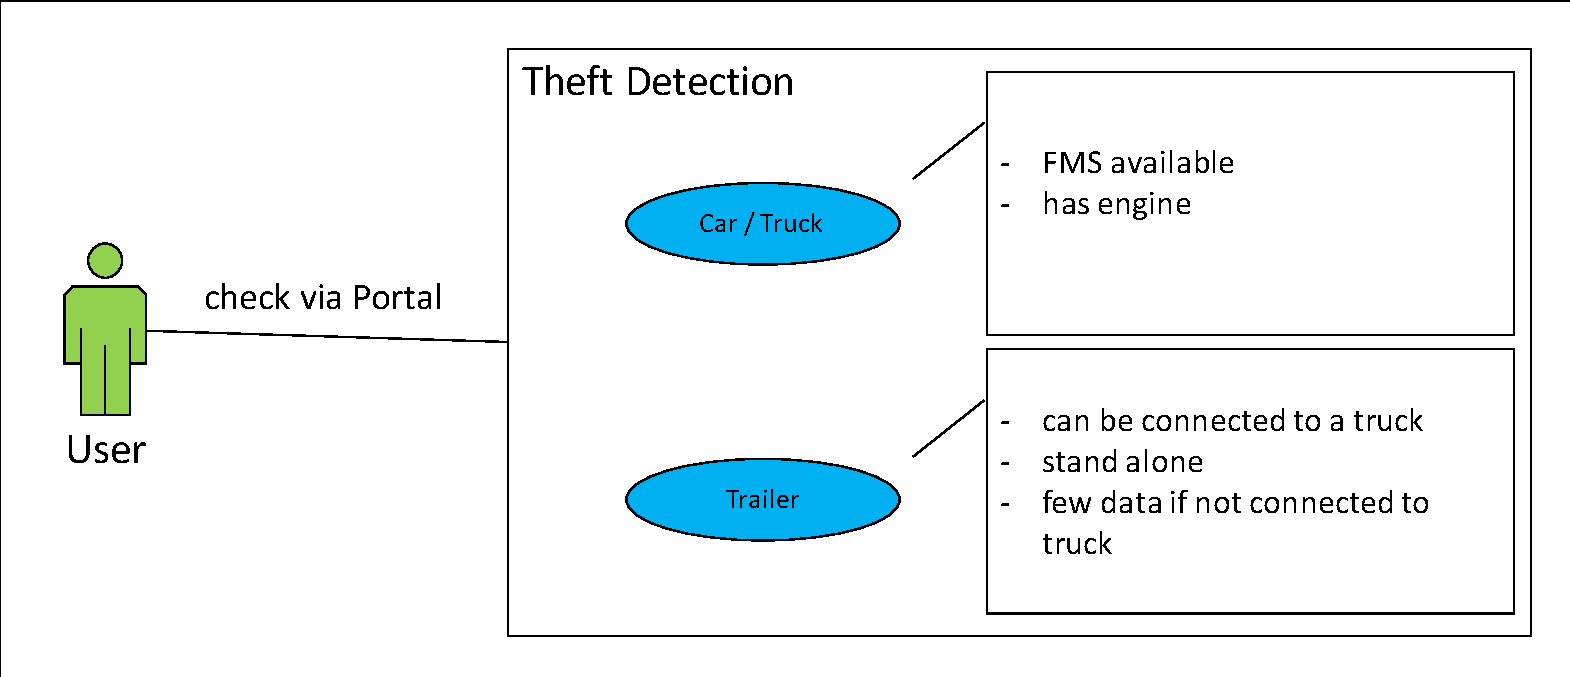
\includegraphics[clip, trim=0.1cm 0.1cm 0.1cm 0.1cm, width=1\textwidth]{src/pic/UseCase}
    \caption{Use Cases}
    \label{fig::useCase}
\end{figure}

We distinct between teft detection for a car or truck and a trailer only because VCGs are often build in trailers. Depending on those configurations we have different data available which have to be considered in the implementation.

\clearpage

\section{Algorithm}
The algorithm works on a principle of the decision tree (see figure \ref{fig::decisionTree}) and it can be used for detecting a theft of either a car/truck or a trailer.

\begin{figure} [h]
    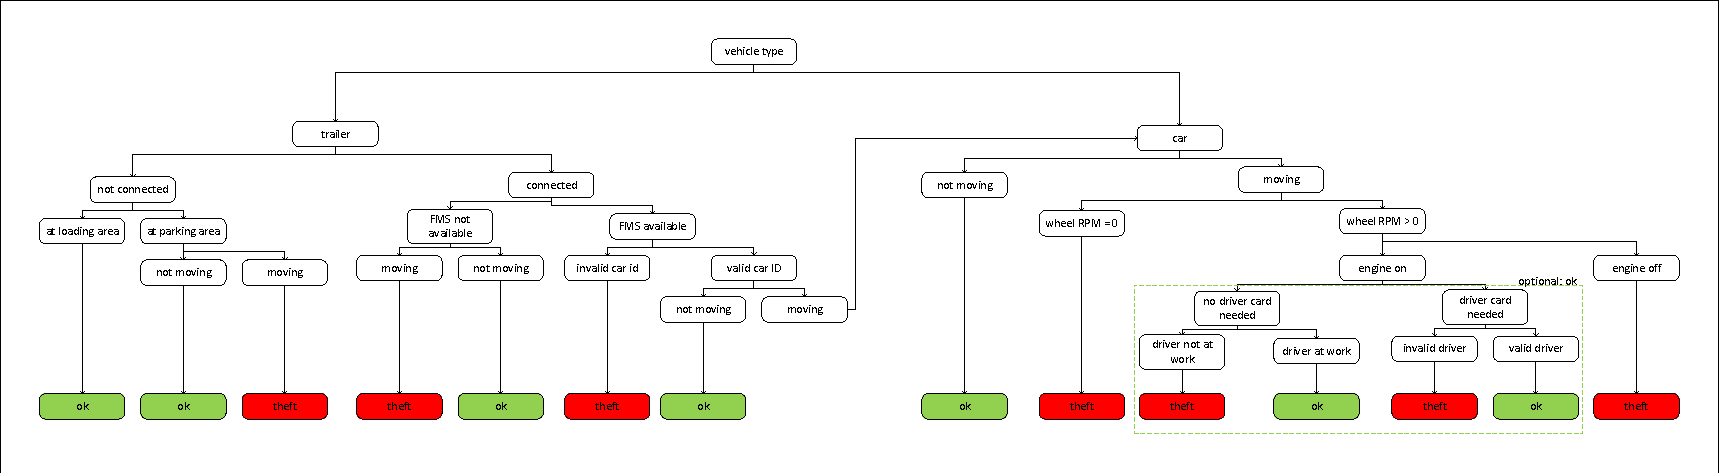
\includegraphics[clip, trim=0.1cm 0.1cm 0.1cm 0.1cm, width=1\textwidth]{src/pic/DecisionTree}
    \caption{Decision tree}
    \label{fig::decisionTree}
\end{figure}

Based on the information whether the specific data is available, the different path in the tree is selected and consequently, the decision is made. Since the use cases for trailer and truck are different, the algorithm will be explained for both cases independently (see figure \ref{fig::decisionTreeTop}).

\begin{figure} [h]
    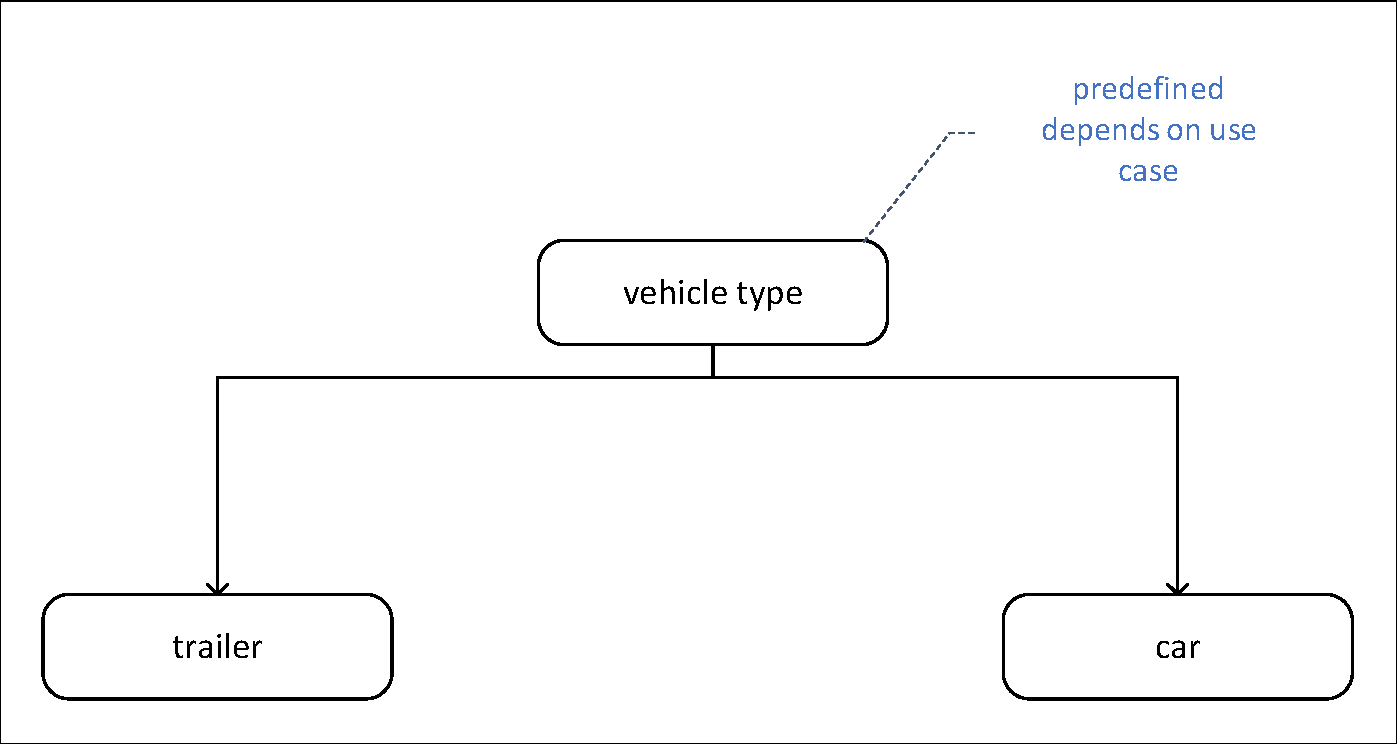
\includegraphics[clip, trim=0.1cm 0.1cm 0.1cm 0.1cm, width=1\textwidth]{src/pic/DecisionTreeTop}
    \caption{Decision tree top}
    \label{fig::decisionTreeTop}
\end{figure}

When the trailer case is considered, there exist specific properties that have to be taken into account in order to distinguish correctly between the possible outcomes. In other words, it has to be determined whether the trailer is connected to a vehicle, whether there is available FMS data, but also the current position of the trailer has to be acquired. 
The first decision is made according to the information of the power connection. If it is the external one, the trailer is not connected, which triggers a query on the current position. Under the assumption that the company that owns the trailer geofenced the loading and parking areas, further decisions are made. On the one side, while the trailer is located within the loading area, no potential theft is detected, regardless of whether the trailer is in motion or not. However, if the trailer is at a parking area, it is assumed that any kind of movement could represent the potential theft and the algorithm will end its path in the "theft detected" final node. The data needed for answering the previously described queries is acquired using the GPS and accelerometer sensors. The GPS is used for collecting the trailer location and checking whether the trailer is in the predefined position. It should be stated that our algorithm can easily be applied to the case when the trailer is being transported by a ship, where the geo-fence can be dynamically generated based on the boat position. When it comes to gathering the movement information, both the GPS and the accelerometer sensors are used. \\
In case that the trailer is connected to the vehicle, one additional resource is used for the algorithm analysis - the FMS data. If this data is not available and the trailer is moving, the theft is obviously detected, because the trailer is attached to an unrecognized vehicle. Again the movement information is acquired from the GPS/accelerometer sensors. However, if the FMS is available, that does not necessarily mean this is an acceptable case because a unique car ID is still to be checked. If it is an invalid id the stealing is detected, otherwise, the information of the vehicle movement is considered. At this point, the algorithm generates queries regarding the vehicle information only, therefore the theft of the car/truck analysis is to be described next and it follows below.

\begin{figure} [h]
    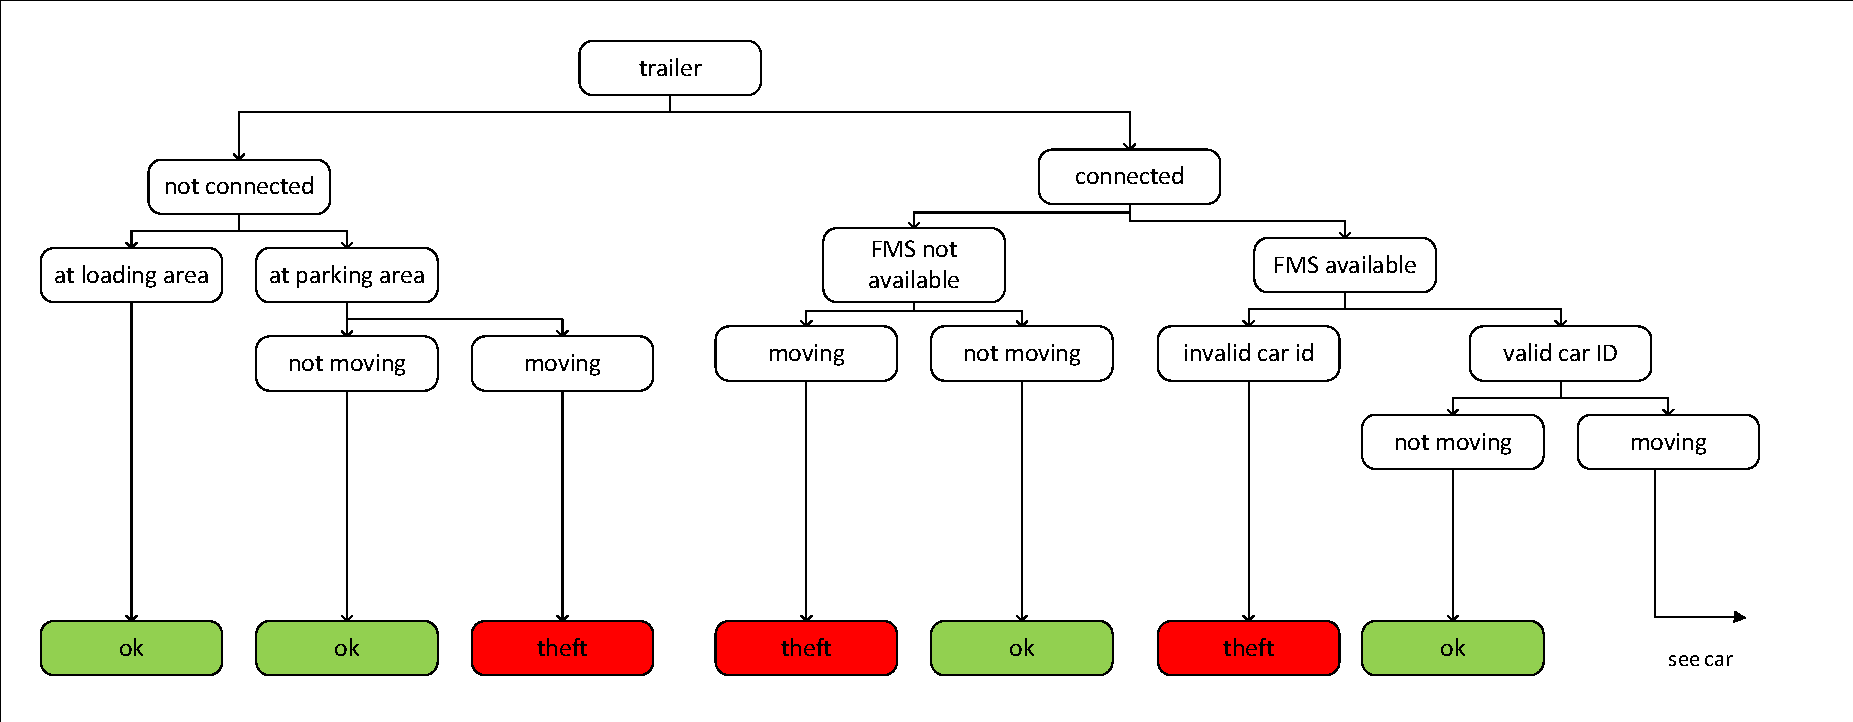
\includegraphics[clip, trim=0.1cm 0.1cm 0.1cm 0.1cm, width=1\textwidth]{src/pic/DecisionTreeTrailer}
    \caption{Decision tree trailer}
    \label{fig::decisionTreeTrailer}
\end{figure}

The GPS/accelerometer sensors answer the first important decision question in this part of the analysis - whether the car is moving or not. It is assumed that no motion represents a valid situation, so the only interesting case is recognizing the theft if there is a movement detected. Therefore, it is henceforth assumed that the vehicle is moving and the rest of the data that determines the path through the tree originates from the FMS. The wheel RPM is the first thing to check in this kind of situation because if the RPM is zero, the car is probably lifted and is being transported illegally. Otherwise, if the wheels are spinning, it should be asserted that the engine is on, which represents a valid scenario. Contrarily, if the engine is off with the RPM greater than zero, the theft is detected.\\
Moreover, if the driver cards are used in a company, the case when the engine is on can be extended in order to provide a more precise outcome. If a driver card is not required, it is checked whether the driver is on a job. If so, it is expected that the driver is in a vehicle, otherwise, the theft is identified. On the other hand, if the driver card is required, information on whether it is an invalid or a valid driver distinguishes between a theft and a regular situation. \\
In section 2.3 it will be explained thoroughly how the main data sources are used.

\begin{figure} [h]
    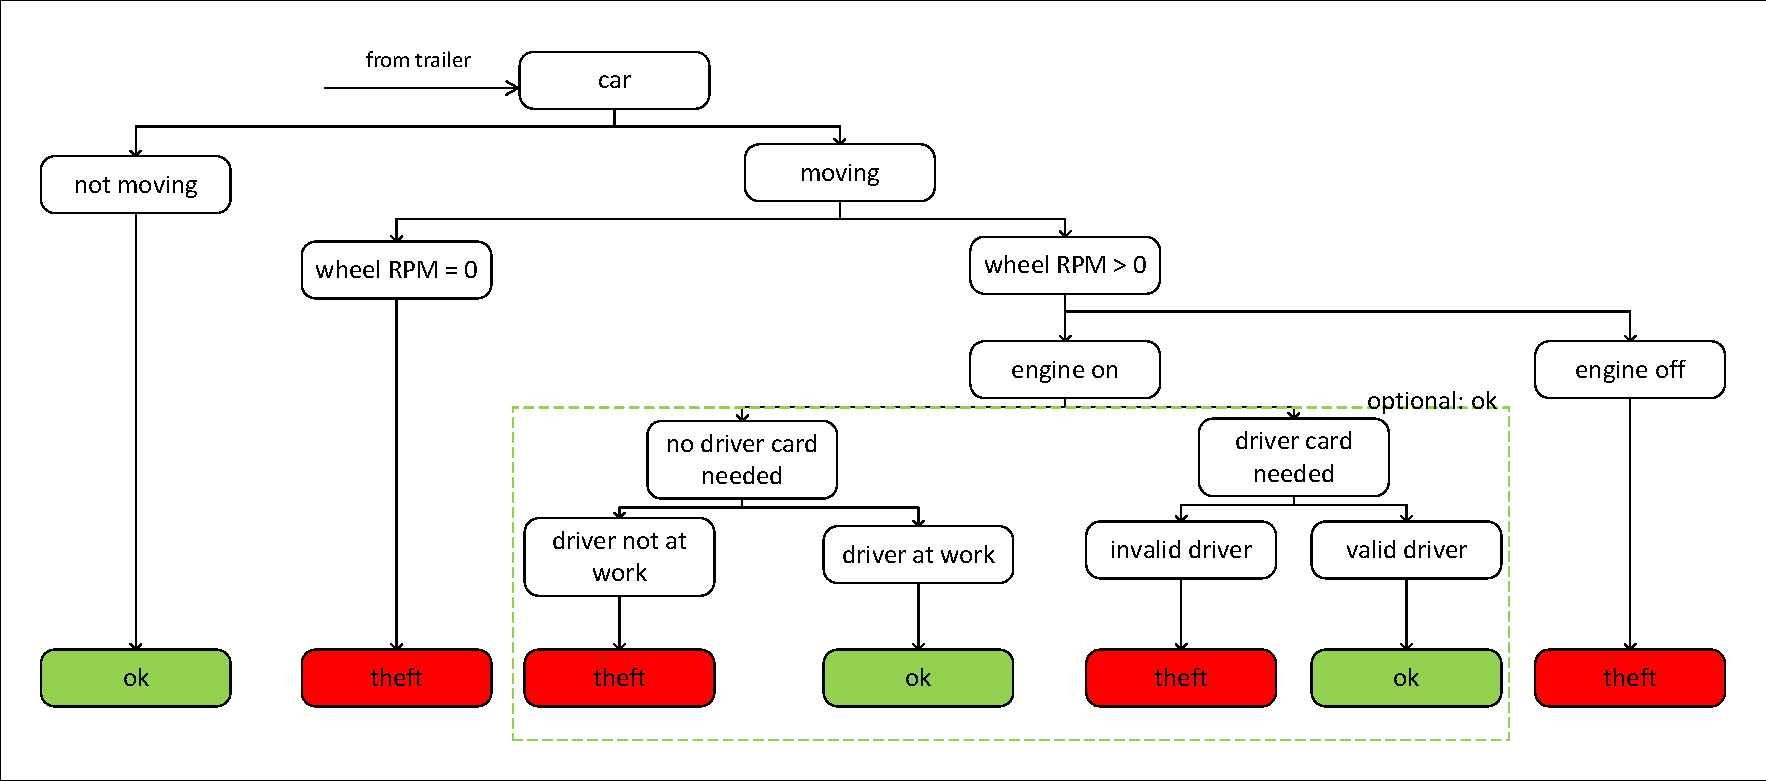
\includegraphics[clip, trim=0.1cm 0.1cm 0.1cm 0.1cm, width=1\textwidth]{src/pic/DecisionTreeCar}
    \caption{Decision tree car}
    \label{fig::decisionTreeCar}
\end{figure}


\clearpage